\documentclass{amsart}
\usepackage{amsmath}
\usepackage{minted}
\usepackage{fancyvrb}
\usepackage{xcolor}
\usepackage{color}
\usepackage{listings}
\usepackage{graphicx}
\usepackage{subfig}
\usepackage{soul}
\newtheorem{theorem}{Theorem}[section]
\newtheorem{lemma}[theorem]{Lemma}

\theoremstyle{definition}
\newtheorem{definition}[theorem]{Definition}
\newtheorem{example}[theorem]{Example}
\newtheorem{xca}[theorem]{Exercise}

\theoremstyle{remark}
\newtheorem{remark}[theorem]{Remark}

\numberwithin{equation}{section}
\lstset{
	basicstyle=\small\ttfamily,
	columns=flexible,
	breaklines=true
}
\setminted[c]{
	frame=lines,
	framesep=2mm,
	baselinestretch=1,
	fontsize=\footnotesize,
	bgcolor=black,
	style=vim,
	linenos
}
\setlength{\textwidth}{\paperwidth}
\addtolength{\textwidth}{-1in}
\calclayout

\makeatletter
\g@addto@macro{\newpage}{\nointerlineskip}
\makeatother



\begin{document}
\vspace*{-80pt}

\title{IMDB Sentiment Analysis}

\author{Luo, Robin (260851506)}
\author{Rousseau, Marc-Andre  (260089646)}
\author{Xu Bide, (260711367)}

\date{\today}
\begin{abstract}
We investigated the predictive power of several well known algorithms to perform sentiment analysis on imdb movie reviews.  Using a linear support vector machine model trained on a dataset of 25000 movies reviews, we were successful in processing the text of a review and predicting whether the review was positive or negative with an accuracy of 91.786 percent on a dataset of 25000 reviews with the true sentiments withheld.  After extensive analysis of various models, we concluded that support vector machine slightly outperformed linear regression which significantly outperformed the Naive Bayes implementation.  The predictive power of a simple support vector machine model including tf-idf, minimal text preprocessing and tetragrams performed extremely well which made it very difficult to determine other features which may have significantly improved predictive power in a less parametrized model.
\end{abstract}
\maketitle
\section{Introduction}
The ubiquity of social networks is no longer a budding phenomenon and is part of the reality in which we now find ourselves.  Many popular sites have included ways for users to share their opinions on a variety of topics and therefore the ability to mine through these posts and determine how users feel about the things being discussed is extremely useful for businesses.  Knowing that a user or group of users desire something or find it appealing creates a market of opportunity for companies in search of low risk opportunities to expand their business operations.  This is one of the most alluring aspects of machine learning.  While the discovery of many of the mathematical underpinnings of machine learning have been discovered for quite some time, it is the rise in computing power which has given us the ability to use these techniques in otherwise intractable situations.  For example gradient descent was invented by the prolific mathematician Augustin-Louis Cauchy in 1847.  For our project, we were given 12500 positive and 12500 negative reviews to train our algorithm and another 25000 to test our code and submit our best guess as to the correct labeling of the test reviews as either positive or negative.  Our best model which used a linear SVM (0.918 accuracy), was much better than Naive Bayes (0.83).
\section{Related Work}
Machine learning and sentiment analysis are hot topics of research with many machine learning conferences having several talks on the topic.  For example, Twitter has been releasing datasets to be mined for things like whether a piece of task is positive, negative or neutral.  Recently, a group of researchers extended this problem to five classification categories and added arabic language content (Rosenthal, 2017).  Many teams submitted ML proposals to classify the twitter posts and the top performing groups used deep neural networks (DNNs) (Rosenthal, 2017).  In addition, out of the top 10 submissions, the second most successful approach to DNNs involved the use of SVMs which is consistent with our best performing model for this project.  A more directly related work involved taking into account sentence negations (Das, 2018).  In this paper, the authors have decided to use a shortcut for negation by negating the word immediately following a negation.  One example of this method would be to take the sentence "I am not happy" which gets converted to "I am not\_happy".  The benefit of this is that by changing only one word, they are able to change the meaning of the entire sentence (Das, 2018).  Our team implemented this feature but it did not have a significant impact on the score after verification by cross-validation and kaggle submission.
\section{Dataset and Setup}
Our training dataset consisted of a list of 25000 reviews properly marked as positive or negative for us to train.  We also had another 25000 data points to test out our model.  The data consist of the content of the reviews and both the training and test sets needed to have their data preprocessed to be able to be consumed by the python libraries.  For the purpose of training and validation, we separated our data into 80\% training and 20\% validation.
\section{Proposed Approach}
The approach we considered is summarized in the following flow chart.  Not all of the elements were eventually considered in our final report since they did not provide any substantial performance benefit above and beyond that which our current models were able to meet.
\begin{figure}
	\centering
	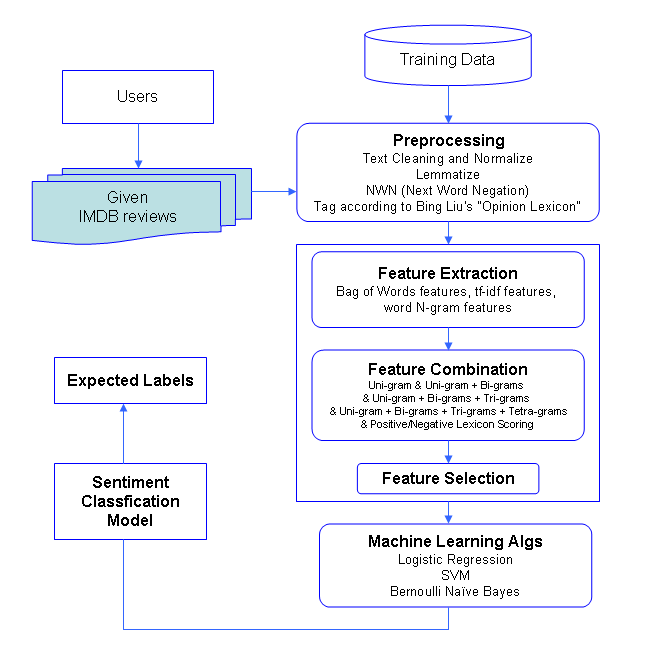
\includegraphics[width=10cm]{fig/flow_chart.png}
	\caption{\textbf{Flow chart of our proposed approach}  The elements that were tested but not ultimately included were the NWN, opinion lexicon tagging as well as the positive and negative lexicon scoring}
	\label{fig:flowchart}
\end{figure}
\subsection{Preprocessing}
For the preprocessing, we considered several models including a raw text input model, a model where the text was cleaned to only include letter characters (LC), a model where the text was processed through a normalization library and the words were separated from the punctuation symbols (SWP), a model with lemmatization (LZ) and a model with next word negation (NWN) from the previously mentioned paper.  For all models with the exception of the raw data, the text was converted to lowercase characters.  Following the initial preprocessing, the data was subsequently tokenized.  For the normalization model, we removed any characters for which the normalization library could not process.  This was usually due to unicode characters which could not be mapped to equivalent ascii characters.
\subsection{Feature, hyperparamter and model selection}
In addition to the features generated by the preprocessing, we used tf-idf and bag of words (BOW) in our pipelines for feature selection.  We implemented SVM, Laplace-smoothed Bernoulli Naive Bayes (NB) and logistic regression (LR) models.  To determine the hyperparameters and for regularization as well as the feature selection, we used a grid-based search algorithm with a cross-validation parameter of 5.  For our BOW feature, we tested out many different values for possible n-gram size and settled with 1-4 after testing out several different options.  For the SVM model, we tried values for the penalty parameter "C" and decided to use the default value of 1.0.  \textbf{In addition to this, once our model was able to associate good or bad to a particular set of words, we used these word to sentiment mappings to analyse subsentences separated by punctuation.  For each bad or good word found, we added 1 or -1 to a counter and then classified the value for the overall text to the sum of all the individual good/bad words found in the text.}  In addition to this, we used a normalization library to standardize the feature vectors so that they had unit length.  In terms of the theoretical underpinnings of the model selection, we used a data-driven approach rather than a conceptual one and so there was little discussion about which model was more appropriate and instead we opted to go with the model that had the best predictive power.
\section{Results}
The task of deciding on a final model based on the performance is quite easy since we only had to code the model and then pick whichever model worked the best, however a discussion of the relative performance of the models is difficult due to how close the top models performed as well as the sheer quantity of possible adjustments.  In general, tf-idf outperformed bag of words, SVM outperformed LR \textbf{and a model allowing for tetragrams outperformed the trigram models.}
\subsection{NB vs LR vs SVM}
The performance of the Naive Bayes was significantly better than a random guess approach but still failed to come close to the performance of the logistic regression or the support vector machine approaches.  One of the fundamental differences between our implementation of Naive Bayes and the \textbf{other two models is that the former does not exclude words whereas the other two had minimum cutoffs for features.  This could account for the performance difference seen between the bag of words LR and the Naive Bayes model.  Our top performing model on cross-validation was a LR model but this did not extend to kaggle submissions for which the SVM slightly outperformed the LR.}
 \subsection{Bag of words vs tf-idf}
The performance of SVM and LR using both BOW and TF-IDF were similar with TF-IDF being slightly better than BOW according to the parameters we chose for min-df and max-df.  For our model, we used a min\_df of 2 and a max\_df of 1.0 meaning that words that appeared in at least 2 of the documents were considered and no constraint was placed on the maximum frequency that a word could occur.  In addition to using these models, we had originally also included stop\_words but these did not show any additional gains above and beyond tf-idf and therefore it would seem as though the idf aspect of the tf-idf implementation may have already been incorporating the information contained in stop\_words by essentially removing those words which were used too frequently by lowering the respective weights.  Looking at the values in Table 1, we can see that for models where BOW and TF-IDF were used, the latter usually performed slightly better.  A strict comparison of these features is difficult due to the many possible parametrizations of the BOW implementation.  Figure 1 shows how the max\_df affects the score and the difference in the score between the BOW and tf-idf be partially due to the inclusion of those common words which appear in almost every paragraph of english ("in","the", etc...).
\begin{figure}
	\centering
	\subfloat[score vs max\_df]{{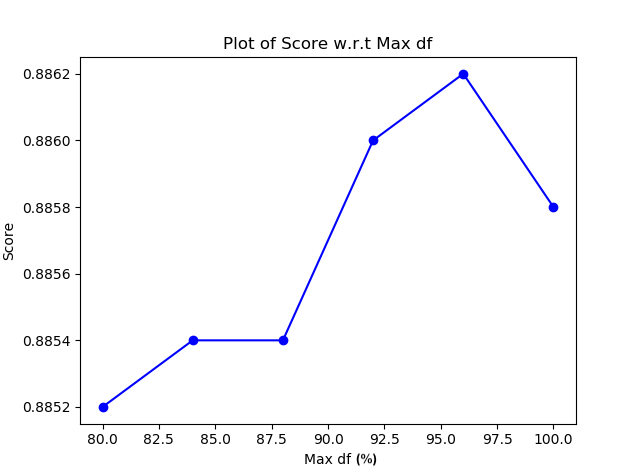
\includegraphics[width=5cm]{fig/max_df_score1.png} }}
	\qquad
	\subfloat[total runtime vs max\_df]{{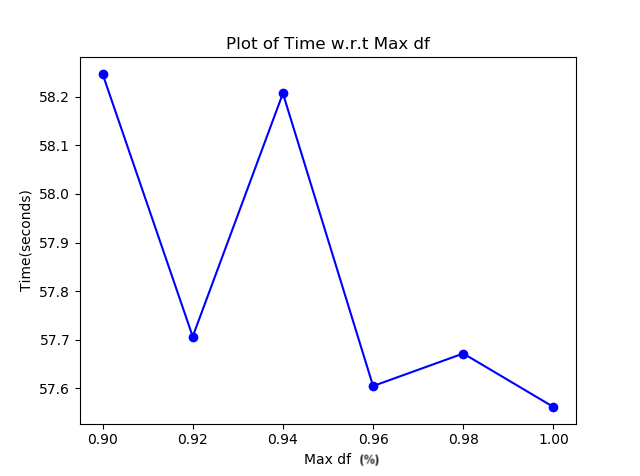
\includegraphics[width=5cm]{fig/max_df_time1.png} }}
	\caption{\textbf{Performance analysis of the max\_df parameter}  In A,  we can see the best prediction is obtained just shy of the 100 percent mark which might account for why our BOW model did slightly worse than the tf\_idf model which would automatically account for the high frequency words.  In (B), we see that above the 90 percent mark, there is little effect on the runtime which coud simply be due to the fact that there are few words which appear extremely frequently and therefore there is no discernable effect on runtime}
	\label{fig:betavsMSE}
\end{figure}
\subsection{N-grams}
We considered many different possibilities for n-grams but ultimately we settled on using (1-4)-grams even though the gain in performance was quite small between limiting ourselves to trigrams and including tetragrams.  The logistic regression model with td-idf showed that the value in increasing above tetragrams was nonexistent.  While the increase in score between the trigram and tetragram models was under 1 percent for most models, the increase seemed consistent across almost all models considered and was therefore included.  The additional value added in considering fourth level n-grams is probably due to common four-word expressions in the english language which convey sentiment.  The low increase in performance is quite simply due to the low frequency of occurrence of these expressions overall for the amount of data we had.
\subsection{Text processing}
The effect of processing and preparing the text was a contributor to performance as can be seen by comparing the values in Table 1.  We can see that by limiting ourselves to letters exclusively, we actually lose some information and the score for the LC models suffered as a result.  As an example, the model using LR, tf-idf and (1-4)-grams had a performance score of 0.895 for the letter character model, a score of 0.913 for the raw text and 0.915 for the model where the text was normalized and converted to lowercase.  The increase in performance between the raw and cleaned data was not universally consistent which could be due to the cleaning removing some information that would otherwise have been useful.  One of the most interesting results is that some of the numbers actually ranked quite high after td-idf weighing and feature weight calculations.  The model which removed everything but letter characters would have removed this important feature and therefore lost some predictive power as a result.
\begin{figure}
	\centering
	\includegraphics[width=10cm]{fig/tf-idfnumber7.jpg}
	\caption{\textbf{Sorted features after tf-idf and training to determine weights.} The number 7 appears to be very strongly associated with a positive review.}
	\label{fig:tfidfnumber7}
\end{figure}
\subsection{Lemmatization}
The non-lemmatized model seemed to perform consistently better than the lemmatized model, however the submission to kaggle suggested that there was in fact a gain in performance in using the lemmatized model.  Lemmatization is a feature which reduces the information rather than increases it and therefore it is not surprising to see some drop in perfomance.  Despite this, the idea behind lemmatization is that there are many words for which only the root of the word conveys information and therefore this should help reduce noise and regularize so as to better extend our model to unseen data.
\subsection{SWP and NWN}
The SWP and NWN models did not seem to provide significant improvements to our model after having already incorporated tf-idf, lemmatize, and a cleaning of the text.  While it is true that our best performing model used SWP (Table 1), this result did not extend into the kaggle submission and could be due to random variance in the data.  We had expected some gain in performance from the NWN and had also tried other forms of regularization of negation but no clear improvement was seen in our kaggle submissions or our cross-validation.  
\section{Discussion and Conclusion}
\subsection{Not losing information when pre-processing}
As we began to work with the data, it became clear that while taking care to properly clean and process the data does provide some benefit, in the presence of powerful features like BOW and tf-idf, giving us a high accuracy, there is very little room for improvement in subtlely massaging the data to make it more suitable.  In addition, preprocessing can actually remove important information as was seen in the table listing the highest weighted words showing the importance of the number 7.  In trying to understand why this might be the case, we browsed metacritic.com to gain some insights into what an average score is and it turns out to be 63/100.  On rotten tomatoes, a fresh review is anything above a 60 whereas a rotten review is anything 59 and below.  It could be that having a user mention the number 7 as being related to how they have rated the movie or how they feel about a movie will more often or not be associated with a positive review since the a leading 7 would be a fair bit higher than the threshold to cross over into a bad review.
\subsection{Difficulty of finding optimization by adding custom features}
In implementing SWP and NWN, we were hoping to see some gains in performance but with a relatively small dataset compared to the number of features, it is difficult to see improvements after having implemented components like tf-idf, bag of words, lemmatize, etc...  To be able to truly create more advanced features, we would either have to consider models that could break down sentence structure or alternatively we could consult someone with domain knowledge of the imdb reviews who could give us insights about how people write their reviews so we could add these to our models.  
\subsection{Capitalization}
While our final model has all words converted to lowercase, it is important to note that there may be a loss of predictive power in doing so.  To be more certain of this, we would have to have a better idea of where the reviews came from.  If the reviews were submitted by users with little to no oversight, then you could expect people writing words in all CAPITAL LETTERS to emphasize a certain point.  This is a potential avenue for further investigation.
\subsection{Domain Knowledge}
While some of us enjoy watching movies, none of the members of our group are experts at reading and analyzing movie reviews and so our analysis is inherently limited to that which someone with a small amount of domain knowledge and a fair bit of computing knowledge can achieve.  In certain situations, having a well informed expert to help guide the machine learning scientist would not only have the potential of improving the performance of the model but it might also help in generating interesting questions of inference about the data.
\section{Future Considerations}
If we were to continue working with the dataset, we might want to consider using a neural network or consider using category theory to better mine sentence structure for important components.  Work involving category theory and natural language processing has been around for many years.  One example being recent work by Kartsaklis et al. (Kartsaklis, 2016).
\section{Division of Work}
\begin{itemize}
\item{\textbf{Robin Luo}}: Model fitting, analysis of the effect of hyperparameters
\item{\textbf{Marc-Andre Rousseau}}: Literature research, TeXing, some minor coding.
\item{\textbf{Peter Xu}}: Coding, feature selection and hyperparameter fitting.
\end{itemize}
\section{References}
\begin{itemize}
	\item [1] Rosenthal, Sara, et al. “SemEval-2017 task 4: Sentiment analysis in Twitter” Proceedings of the 11th International Workshop on Semantic Evaluations (SemEval-2017), pp. 502–518.
	\item [2] Das, Bijoyan. Chakraborty, Sarit. "An improved text sentiment classification model using tf-idf and next word negation" June, 2017, eprint arXiv:1806.06407
	\item [3] Kartsaklis, D., Sadrzadeh, M., Pulman, S., \& Coecke, B. (2016). Reasoning about meaning in natural language with compact closed categories and Frobenius algebras. In J. Chubb, A. Eskandarian, \& V. Harizanov (Eds.), Logic and Algebraic Structures in Quantum Computing (Lecture Notes in Logic, pp. 199-222). Cambridge: Cambridge University Press. doi:10.1017/CBO9781139519687.011
\end{itemize}
\section{Appendix}
\begin{center}
	\begin{table}
		\caption{Runtime and F1 performance analysis of various models} \label{tab:title}
		\begin{tabular}{|| c | c | c | c | c | c ||}
			\hline
			Number & Model & F1-score & \#features & Fit runtime (s) & Prediction runtime (s) \\
			\hline\hline
			1 & Bernoulli NB + BOW & 0.84879 & 67708 & 1020 & 5520 \\
			\hline
			2 & LR,LCs, 1-gram & 0.88561 & 27254 & 10 & 2 \\
			\hline
			3 & LR, BOW, LCs, (1-4)-gram &  0.88961 & 104211 & 106 & 7 \\
			\hline
			4 & LR, tf-idf, LCs, (1-4)-gram & 0.89481 & 104211 & 95 & 6 \\
			\hline
			5 & LR, tf-idf, raw, 1-gram & 0.88541 & 27745 & 29 & 4 \\
			\hline
			6 & LR, BOW, raw, (1-2)-gram & 0.89521 & 166041 & 54 & 9 \\
			\hline
			7 & LR, BOW, raw, (1-3)-gram & 0.89601 & 290118 & 114 & 14 \\
			\hline
			8 & LR, BOW, raw, (1-4)-gram & 0.89521 & 342886 & 230 & 230 \\
			\hline
			9 & LR, tf-idf, raw, 1-gram & 0.89181 & 27745 & 20 & 6 \\
			\hline
			10 & LR, tf-idf, raw, (1-2)-gram & 0.90881 & 166041 & 55 & 8 \\
			\hline
			11 & LR, tf-idf, raw, (1-3)-gram & 0.91161 & 290118 & 110 & 10 \\
			\hline
			12 & LR, tf-idf, raw, (1-4)-gram & 0.91301 & 342886 & 199 & 20 \\
			\hline
			13 & LR, tf-idf, raw, (1-5)-gram & 0.91301 & 358250 & 211 & 13 \\
			\hline
			14 & LR, tf-idf, cleanup, (1-3)-gram & 0.91381 & 284493 & 116 & 12 \\
			\hline
			15 & LR, tf-idf, cleanup, (1-4)-gram & 0.91581 & 334013 & 169 & 18\\
			\hline
			16 & LR, tf-idf, cleanup, SWP, (1-3)-gram & 0.91441 & 284955 & 117 & 10 \\
			\hline
			17 & \textbf{LR, tf-idf, cleanup, SWP, (1-4)-gram} & \textbf{0.91561} & \textbf{333673} & \textbf{166} & \textbf{20} \\
			\hline
			18 & LR, tf-idf, cleanup, lemmatize, (1-3)-gram & 0.91161 & 283063 & 108 & 11\\
			\hline
			19 & LR, tf-idf, cleanup, lemmatize, (1-4)-gram & 0.91281 & 334089 & 178 & 12 \\
			\hline
			20 & LR, tf-idf, cleanup, NWN, (1-3)-gram & 0.91381 & 264522 & 89 & 9\\
			\hline
			21 & LR, tf-idf, cleanup, NWN, (1-4)-gram & 0.91441 & 297461 & 147 & 11\\
			\hline
			22 & LR, tf-idf, cleanup, Lemmatize, SWP (1-3)-gram & 0.91201 & 283682 & 85 & 8 \\
			\hline
			23 & LR, tf-idf, cleanup, Lemmatize, SWP (1-4)-gram & 0.91241 & 333997 & 141 & 11\\
			\hline
			24 & LR, tf-idf, cleanup, Lemmatize, SWP, NWN, (1-3)-gram & 0.91281 & 263993 & 90 & 9 \\
			\hline
			25 & LR, tf-idf, cleanup, Lemmatize, SWP, NWN, (1-4)-gram & 0.91261 & 298356 & 132 & 10\\
			\hline
			26 & SVM, tf-idf, raw, (1-4)-gram & 0.91521 & 1010594 & 167 & 13 \\
			\hline
			27 & SVM, tf-idf, cleanup, (1-4)-gram & 0.91501 & 987640 & 155 & 15 \\
			\hline
			28 & SVM, tf-idf, cleanup, NWN, (1-4)-gram & 0.91401 & 899187 & 156 & 12\\
			\hline
			29 & \textbf{SVM, tf-idf, cleanup, Lemmatize, (1-4)-gram} & \textbf{0.91321} & \textbf{987519} & \textbf{171} & \textbf{12}\\
			\hline
			30 & SVM, tf-idf, cleanup, SWP, (1-4)-gram & 0.91481 & 988012 & 161 & 16\\
			\hline
			31 & SVM, tf-idf, cleanup, SWP, Lemmatize, NWN, (1-4)-gram & 0.91541 & 901848 & 164 & 13\\
			\hline\hline
		\end{tabular}
		\caption*{\textbf{Summary of selected models considered for our final submission.} The final model performance was determined via a study of the effect of modifying the parameters on the F1-scores.  All runtimes with the exception of the Naive Bayes did not preclude extensive testing.  A subset of the models under consideration have been presented.  Our best performing model on the cross validation as well as the best performing model on kaggle are in bold.}
	\end{table}
\end{center}
\end{document}
